%%%%%%%%%%%%%%%%%%%%%%%%%%%%%%%%%%%%%%%%%%%%%%%%%%%%%%%%%%%%%%%%%%%%%%%%%%%%%%%%
\section{Getting Started with Snakemake}

%%%%%%%%%%%%%%%%%%%%%%%%%%%%%%%%%%%%%%%%%%%%%%%%%%%%%%%%%%%%%%%%%%%%%%%%%%%%%%%%
\begin{frame}
    \frametitle{Outline}
    \begin{columns}[t]
        \begin{column}{.5\textwidth}
            \tableofcontents[sections={1-9},currentsection]
        \end{column}
        \begin{column}{.5\textwidth}
            \tableofcontents[sections={10-18},currentsection]
        \end{column}
    \end{columns}
\end{frame}

%%%%%%%%%%%%%%%%%%%%%%%%%%%%%%%%%%%%%%%%%%%%%%%%%%%%%%%%%%%%%%%%%%%%%%%%%%%%%%%%
\begin{frame}
	\frametitle{What is this about?}
	\begin{question}[Questions]
		\begin{itemize}
			\item How can workflow development be started?
			\item What is a good directory layout?
			\item How does a workflow description look like?
		\end{itemize}
	\end{question}
	\begin{docs}[Objectives]
		\begin{enumerate}
			\item Introduce you to conceptualization
			\item First demonstration of directory layouts
			\item Introducing a first (very basic) workflow
		\end{enumerate}
	\end{docs}
\end{frame}

\subsection{Tasksetting}

%%%%%%%%%%%%%%%%%%%%%%%%%%%%%%%%%%%%%%%%%%%%%%%%%%%%%%%%%%%%%%%%%%%%%%%%%%%%%%%%
\begin{frame}
  \begin{figure}
    \centering
    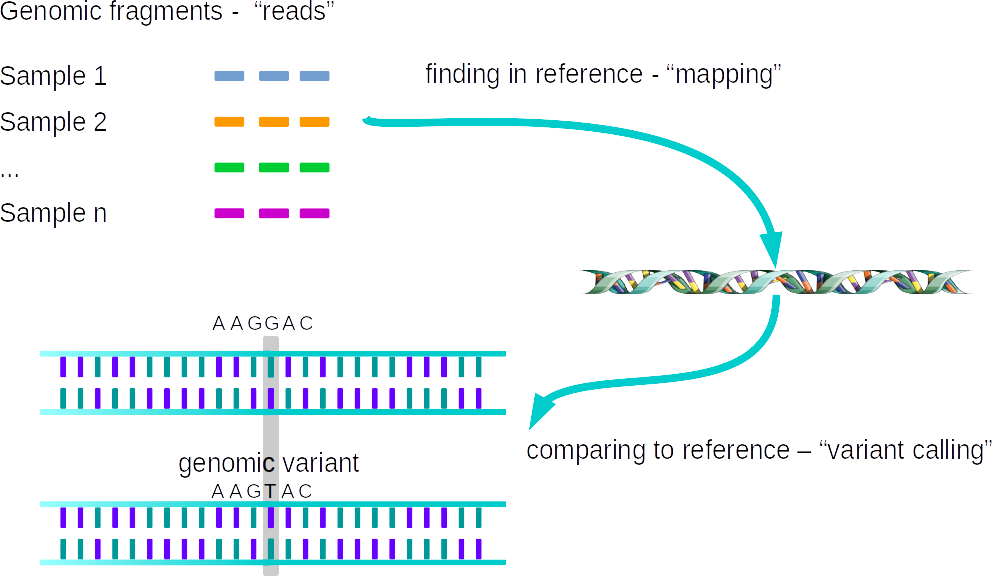
\includegraphics[width=0.95\textwidth]{biology/variant_calling_workflow.png}
  \end{figure}
\end{frame}

%%%%%%%%%%%%%%%%%%%%%%%%%%%%%%%%%%%%%%%%%%%%%%%%%%%%%%%%%%%%%%%%%%%%%%%%%%%%%%%%
\begin{frame}[fragile]
  \frametitle{Getting the Tutorial Data}
  \begin{alertblock}{This is Subject to Change!}
   This tutorial carries a bug in \texttt{bioconda}: A certain piece of software is not compatible
   with the current version of Python. Hence, we run a script (we will look into it), which downloads
   our data and downgrades Python, such that everything will be working.\newline
   \textbf{Of course, this might all not be necessary in a future course.}
  \end{alertblock}
  \pause
  For the tutorial we run:
  \begin{lstlisting}[language=Bash, style=Shell]
$ bash setup/02_tutorial_setup.sh
  \end{lstlisting}
\end{frame}

%%%%%%%%%%%%%%%%%%%%%%%%%%%%%%%%%%%%%%%%%%%%%%%%%%%%%%%%%%%%%%%%%%%%%%%%%%%%%%%% 
\begin{frame}[fragile]
  \frametitle{The Setup Script}
  \begin{lstlisting}[language=Bash, style=Shell, basicstyle=\tiny]
# 0. we are going to use ONE environment with the same
#    name as the workflow we are going to create
NAME="snakemake-tutorial"

# 1. On many HPC systems we are going to install via a proxy.
#    This might ignore TLS, hence we turn off all warnings.
#    Note: TLS might still be used, but not ALL proxies use it.
export PYTHONWARNINGS="ignore:Unverified HTTPS request"

# 1. create the environment for the tutorial
mamba create --name $NAME

# 2. activate the environment
mamba activate $NAME

# TODO: This step is necessary because of the outdated 
#       setup, where Python >= 3.10 does not work
#       with pysam
mamba install Python=3.9
  \end{lstlisting}
  Here we create an environment, activate it and install an older version of Python. Questions to the code?
\end{frame}

%%%%%%%%%%%%%%%%%%%%%%%%%%%%%%%%%%%%%%%%%%%%%%%%%%%%%%%%%%%%%%%%%%%%%%%%%%%%%%%% 
\begin{frame}[fragile]
  \frametitle{Getting the example Data}
  Again we are using a script to download and extract our example data. Please run
  \begin{lstlisting}[language=Bash, style=Shell]
$ bash setup/03_get_data.sh
  \end{lstlisting}
  Subsequently change into the directory \altverb{snakemake-tutorial} which has been created. 
  \pause
  \begin{question}
  	Which files do you find?
  \end{question}
\end{frame}

%%%%%%%%%%%%%%%%%%%%%%%%%%%%%%%%%%%%%%%%%%%%%%%%%%%%%%%%%%%%%%%%%%%%%%%%%%%%%%%% 
\begin{frame}[fragile]
  \frametitle{The Collector Script}
  \begin{lstlisting}[language=Bash, style=Shell, basicstyle=\tiny]
#!/bin/bash

# 1. we are going to work in a dedicated directory:
mkdir snakemake-tutorial && cd snakemake-tutorial

# 2. download the sample data
echo "downloading sample data"
curl -L https://api.github.com/repos/snakemake/snakemake-tutorial-data/tarball -o snakemake-tutorial-data.tar.gz

# 3. unpack the sample data
echo "unpacking sample data"
tar --wildcards -xf snakemake-tutorial-data.tar.gz --strip 1 "*/data" "*/environment.yaml"

# 4. this is necessary, because we need a simple list of packages
#    after we downgraded the python version in the step afore.
@cat environment.yaml | tail -n+5 | cut -c5- > environment2.txt@

# 5. install all necessary software
mamba install --file environment2.txt
  \end{lstlisting}
  \begin{block}{Two Notes}
    \begin{enumerate}
     \item The tinkering in step 4 is so weird, due to the reasons explained.
     \item You can install software from a) a simple text file, b) during creation of the environment and c) let \texttt{snakemake} do it for you (introduced later).
    \end{enumerate}
  \end{block}
\end{frame}

%%%%%%%%%%%%%%%%%%%%%%%%%%%%%%%%%%%%%%%%%%%%%%%%%%%%%%%%%%%%%%%%%%%%%%%%%%%%%%%% 
\begin{frame}[fragile]
  \frametitle{Installing Software \emph{with} Conda - Using Environments II}
  Using our new environment we can activate it:
  \begin{lstlisting}[language=Bash, style=Shell]
$ mamba activate snakemake-tutorial
  \end{lstlisting}
  and install ``\texttt{snakemake}'' by running
  \begin{lstlisting}[language=Bash, style=Shell]
$ mamba install snakemake
  \end{lstlisting}
  Now, we are all set. 
  \begin{hint}
  	Just that you know: ``\texttt{snakemake}'' is able to install the requested software for you!
  \end{hint}
\end{frame}

%TODO: Once VSC is running on logins, we should change this slide
%%%%%%%%%%%%%%%%%%%%%%%%%%%%%%%%%%%%%%%%%%%%%%%%%%%%%%%%%%%%%%%%%%%%%%%%%%%%%%%
\begin{frame}[fragile]
  \frametitle{We are almost there \ldots}
  In order to start working, we need an editor.
  \begin{itemize}[<+->]
   \item load your editor \altverb{geany} or \altverb{gedit} \emph{before} attempting to load modules in the same shell. Start it like
         \begin{lstlisting}[language=Bash, style=Shell]
$ geany & 
         \end{lstlisting}
   \item Best use a terminal multiplexer \textbf{or} multiple logins (otherwise you have to develop and execute in one shell).
  \end{itemize}
\end{frame}



